\documentclass[assd_tp3_main.tex]{subfiles}
\usepackage{graphicx}

\begin{document}

\section{Placa Base ADA}
\subsection{Acondicionamiento de la señal}
Dado que el conversor ADC trabaja únicamente con señales positivas, es necesario agregar un offset a la señal de entrada, para aprovechar la máxima excursión del integrado. Como los integrados de los filtros no pueden trabajar con señales de más de 5V, se eligió un offset de 2.5V y la señal queda limitada a $5V_{pp}$. El circuito implementado es el siguiente:

\begin{figure}[H]
	\centering
	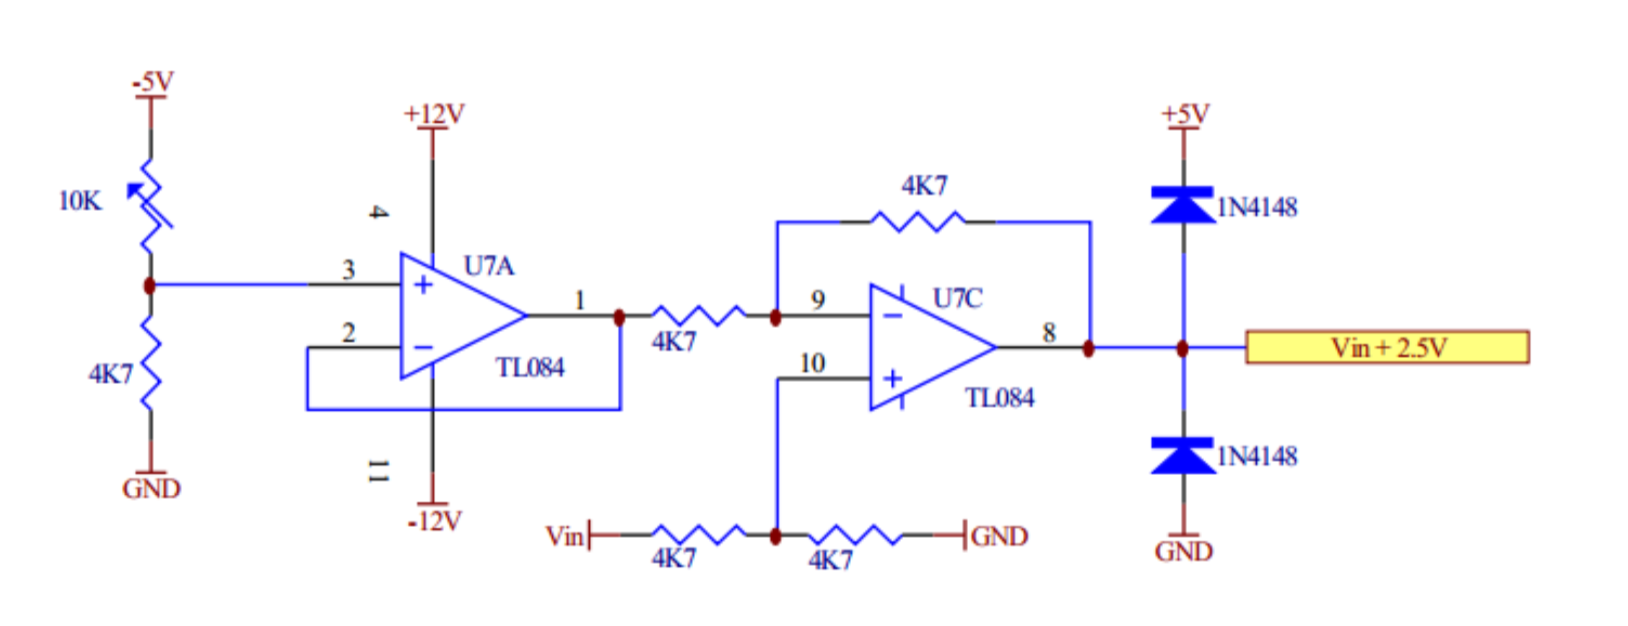
\includegraphics[width=0.6 \textwidth]
	{images/ej1/offset.png}
	\caption{Circuito de Offset}
	\label{fig:offset}
\end{figure}

\subsection{Conversor analógico - digital}
Se utilizó el integrado ADC0809, un conversor analógico-digital de 8 bits, compuesto
por tres partes principales: una escalera de resistencias, un registro de aproximación
sucesivo y un comparador.
Al recibir un flanco ascendente de START, el registro del conversor se restablece, la
señal de fin de la conversión (EOC) se mantiene alta por un tiempo denominado $t_{EOC}$
(EOC Delay Time) para después pasar a su estado bajo como se muestra en la
figura \ref{fig:ADC}. La conversión se inicia entre 0 y 8 ciclos de clock luego del flanco descendente de START. Luego, para avisar la finalización de la conversión, la señal de
EOC vuelve a su estado alto.
Para realizar sucesivas conversiones, en la hoja de datos se recomienda unir la salida
de la señal EOC a la entrada del START, logrando que el conversor reciba como nuevo
pulso de START al flanco ascendente de la señal EOC y comience una nueva
conversión. Si se utiliza en este modo, un pulso de inicio de conversión externo debe
aplicarse después de encenderse.
Es importante que durante todo el tiempo de conversión la señal analógica de entrada
se mantenga estable para asegurar que la misma se efectúe de manera correcta. 

\begin{figure}[H]
	\centering
	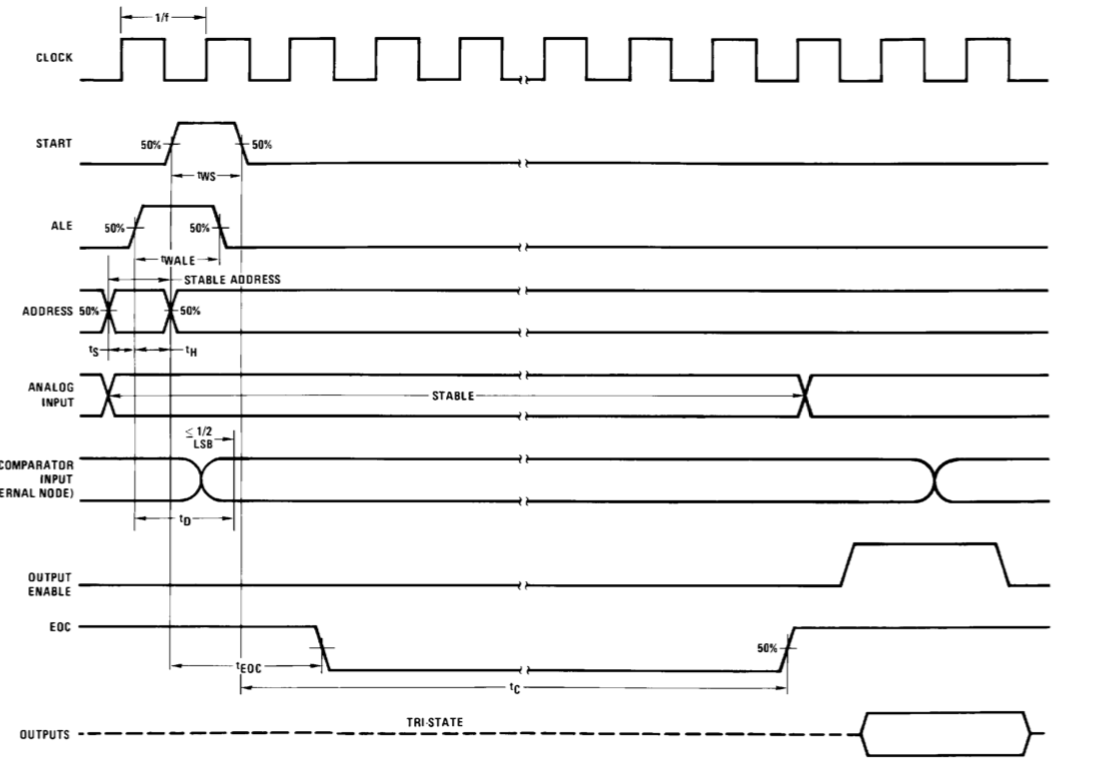
\includegraphics[width=0.4 \textwidth]
	{images/ej1/adcsignals.png}
	\caption{Señales ADC}
	\label{fig:ADC}
\end{figure}

A una frecuencia de clock de 640KHz, el ADC0809 requiere 100 $\mu$s para realizar la conversión. No será necesario el uso de un Sample \& Hold si la entrada varía menos de 1 bit en ese tiempo, pero en caso contrario, cuando la entrada varíe rápidamente si lo será, y se sincroniza al mismo con la señal de EOC. La señal de EOC bajará entre 0 y 8 pulsos de clock después del flanco ascendente de START. Puede pasar que el tiempo de sample (cuando EOC está en su estado alto) sea menor al tiempo de transitorio del Sample \& Hold, haciendo que el valor guardado en
el hold un valor incorrecto.
Como solución a esto se decidió no utilizar la conexión propuesta en la hoja de datos,
si no que se conectó el START y el EOC al FPGA. Utilizando un clock a la frecuencia de
muestreo, en cuanto llega un flanco ascendente del clock el sample and hold se pone
en estado hold y luego de 8$\mu$ s (que es el tiempo de establecimiento) se manda el
START al ADC. Cuando se finaliza la conversión, el EOC pasa a estado alto y el sample
and hold al estado sample y se actualiza la salida del flip flop. Una vez en este estado
se espera al flanco ascendente del clock y se repite el ciclo.
El clock del flip flop está conectado al EOC para que la salida se actualice una vez que
se haya terminado la conversión. 

\subsection{Conversor digital - analógico}

Se utilizó el integrado DAC0800, un conversor D/A de 8 bits con salida diferencial de
corriente. Para convertirlo a un nivel de tensión se utilizó el circuito propuesto por la
hoja de datos que se muestra a continuación:

\begin{figure}[H]
	\centering
	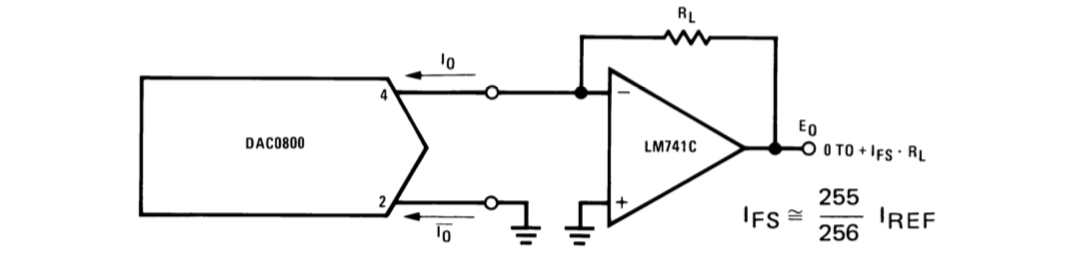
\includegraphics[width=0.6 \textwidth]
	{images/ej1/dac.png}
	\caption{Configuración DAC}
	\label{fig:DAC}
\end{figure}

La salida va de 0 a $V_{fs} = I_{fs}R_f$. 

\subsection{Filtros}
Para implementar los filtros antialiasing y recuperador, se utilizó el integrado MAX297.
Éste funciona como un filtro pasa bajos Cauer de orden 8 que funciona con capacitares switcheados. El dispositivo permite ajustar la frecuencia de paso del filtro
mediante dos formas: la primera mediante capacitares externos que ajustan al
oscilador interno del integrado, y la segunda, con un clock externo que tiene una
frecuencia proporcional a la frecuencia de paso.
En este caso se decidió utilizar la segunda opción, y más adelante se hará el cálculo
de la frecuencia que debe tener el clock para ajustar bien la frecuencia de paso del
filtro.
A continuación se estudiará la función transferencia analógica del integrado para
luego hallar la transformación de s$\rightarrow$z. A partir de las características del integrado

\subsubsection{Cálculo de la frecuencia del clock externo}

Según la hoja de datos del integrado la relación de la frecuencia del clock y la frecuencia de paso es: 

\begin{equation}
	\frac{f_{clk}}{f_p} = 50
	\label{eq:fpfclk}
\end{equation} 

Donde la frecuencia de paso puede ir de 0.1Hz a 50KHz. En la banda de paso hay un
ripple típico de 0.23 dB medidos a una $f_{clk}=50KHz$ y una atenuación en la banda
atenuada de 80dB. A continuación se muestra la respuesta en frecuencia del filtro dada
para una frecuencia de paso de 1KHz: 

\begin{figure}[!ht]
\begin{centering}
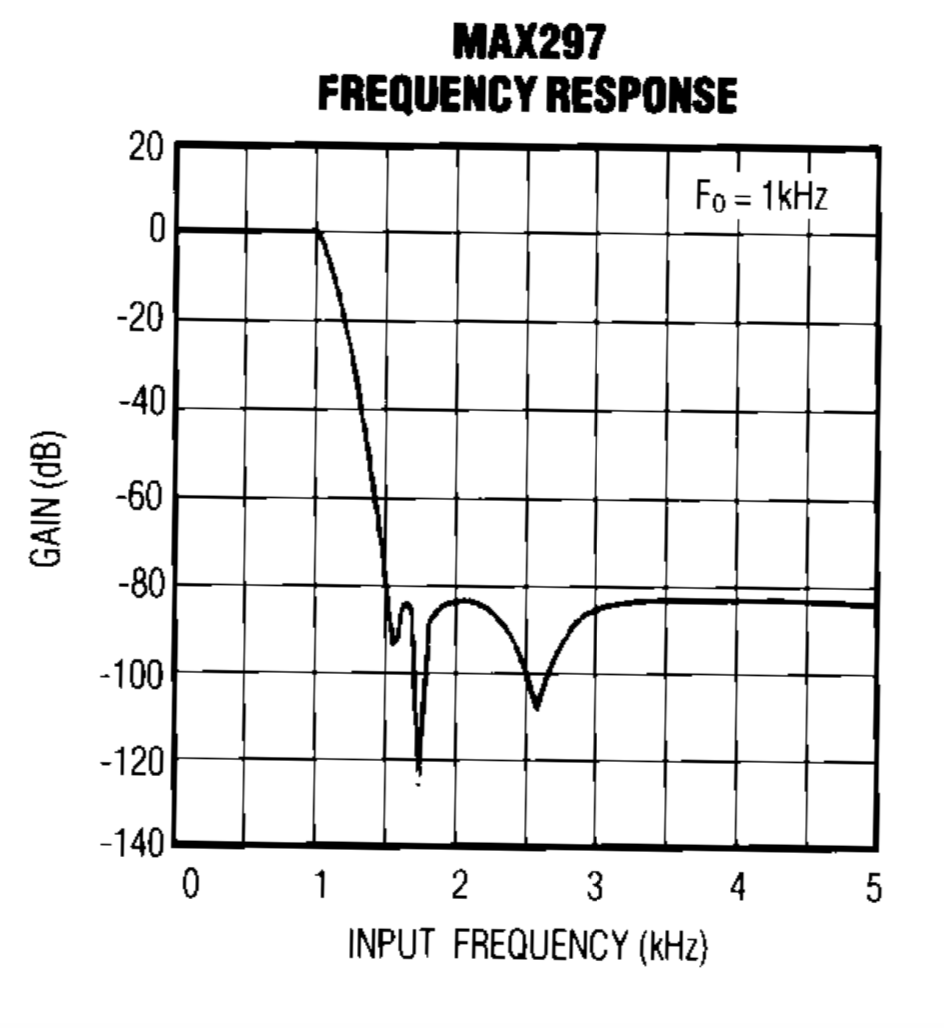
\includegraphics[scale=0.2]{images/ej1/tf.png}
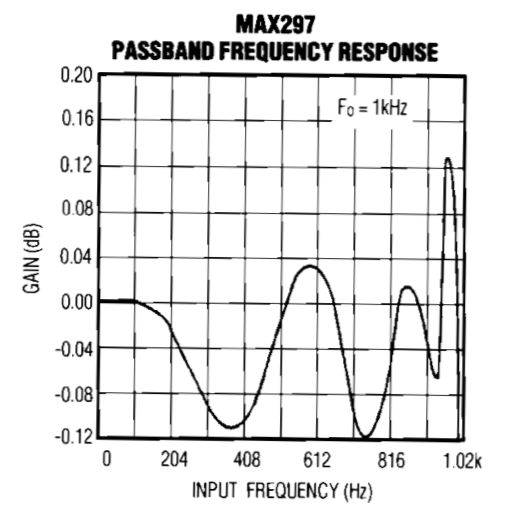
\includegraphics[scale=0.4]{images/ej1/tfpaso.png}
\par\end{centering}
\caption{Respuesta en frecuencia del integrado MAX297}
\end{figure}

Dado que se pide muestrear con frecuencias entre 6KHz y 44.5KHz, para que no se
produzca aliasing, por le criterio de Nyquist la frecuencia de atenuación deberá ser:
$$ f_{a} = \frac{f_s}{2}$$

Por lo que debería suceder que comprenda el intervalo entre 3KHz y 22.25KHz.
Y como la selectividad esta dada por:
$$\frac{f_a}{f_p}=1.5$$
$$f_p = \frac{f_s}{3}$$


Sabiendo la relación entre la frecuencia del clock y la frecuencia de paso dada por la
ecuación \ref{eq:fpfclk}, se obtiene finalmente:

$$ f_{clk} = \frac{50}{3}f_s \simeq 16f_s$$

Entonces queda que el rango de las frecuencias de clock deberá ser: 

$$ 48KHz \leq f_{clk} \leq 712KHz $$

\subsubsection{Alimentación y protecciones}
La alimentación del integrado se encuentra acotada entre $\pm 2.35V$ y $\pm6V$ Dual Supply,
en este caso se alimentó con $\pm5V$. Por lo que se decidió poner diodos zener de 5.6V
conectados como muestra la figura. Luego en caso de que se coloque la alimentación
al revés, actúan los diodos que limitan la tensión a 0.7V protegiendo al integrado.
Además como el integrado suele quemarse con los picos de corriente que resultan del
encendido de la fuente se colocó un capacitar para evitarlas y además una resistencia
para que el capacitar pueda descargarse. 

\begin{figure}[H]
	\centering
	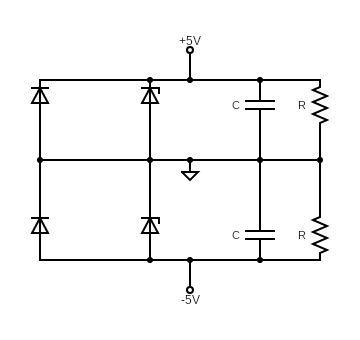
\includegraphics[width=0.6 \textwidth]
	{images/ej1/proteccion alim.png}
	\caption{Protección en la alimentación}
	\label{fig:pal}
\end{figure}

La entrada analógica tampoco debe sobrepasar los límites permitidos
$(V^- - 0.3V \leq Vin \leq V^+ + 0.3V )$, por lo que se colocó la siguiente protección:

\begin{figure}[H]
	\centering
	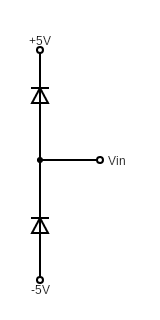
\includegraphics[width=0.2 \textwidth]
	{images/ej1/proteccion in.png}
	\caption{Protección en la entrada}
	\label{fig:pin}
\end{figure}



\end{document}
